\chapter{Introduction}



\section{Project domain - Self-Sovereign Identity (SSI)}

\paragraph{}
On April 25th 2016, Chirstopher Allen launched a blog-post laying out his vision for the future of digital identity titled "The Path to Self-Sovereign Identity"\cite{ThePathToSelfSovereignIdentity}. 

Allen's vision sees \acrfull{ssi} as the final step in the evolution of digital identity: "The models for online identity have advanced through four broad stages since the advent of the Internet: centralized identity, federated identity, user-centric identity, and self-sovereign identity."\cite{ThePathToSelfSovereignIdentity}

In the following years a whole array of new open-source technologies have initiated research and development into realizing Allen's vision. 

\acrfull{dids} is a core \acrshort{ssi}-technology, and it's \textit{design goals}\cite{DIDDesignGoals} gives us a hint about which problems \acrshort{ssi} is trying to solve:
\begin{description}
    \item["Decentralization:] Eliminate the requirement for centralized authorities or single point failure in identifier management, including the registration of globally unique identifiers, public verification keys, services, and other information."
    \item["Control:] Give entities, both human and non-human, the power to directly control their digital identifiers without the need to rely on external authorities."
    \item ["Privacy:] Enable entities to control the privacy of their information, including minimal, selective, and progressive disclosure of attributes or other data."
\end{description}

\paragraph{}
To understand this work, you should at least have a surface-level understanding of the following three core SSI-technologies - \acrfull{dids}, \acrfull{didcomm} and \acrfull{vc} - and how they relate to one another. This chapter will give you a brief summary of all three of them, beginning with \acrshort{dids}:

\newpage




\subsection{Decentralized Identifiers (DIDs)} 

According to \textit{DID Use Cases}\cite{DIDUseCases}, a \acrshort{did} is "a new type of identifier that has 4 essential characteristics:"
\begin{description}
    \item["1. decentralized:] There should be no central issuing agency;"
    \item["2. persistent:] The identifier should be inherently persistent, not requiring the continued operation of an underling organization;"
    \item["3. cryptographically verifiable:] It should be possible to prove control of the identifier cryptographically"
    \item["4. resolvable:] It should be possible to discover metadata about the identifier.
\end{description}
    
\paragraph{}
There are many different types of \acrshort{dids} that fit these characteristics. A specific type of \acrshort{did} is called a \gls{did-method}\cite{DIDMethod}. Each \gls{did-method} provides a unique specification on how to perform the different \gls{did-method-operations}\cite{DIDMethodOperations} - Create, Resolve, Update, Deactivate. 

\paragraph{}
The simplest \gls{did-method} is called \gls{did-key}\cite{DIDKey}. \gls{did-key} is created by generating a cryptographic public-private keypair on your machine, and using the public part of the keypair as a base for the DID.

\begin{lstlisting}[caption={Example of a \gls{did-key}}]
did:key:z6MkpTHR8VNsBxYAAWHut2Geadd9jSwuBV8xRoAnwWsdvktH  <--- Public key
\end{lstlisting}

If you stumble upon a \acrshort{did} in the wild, it should be easy to recognize it as a \acrshort{did}, because they all share the same signature.

\begin{lstlisting}[caption={DID-signature}]
did:<method>:<unique method-specific string of characters>
\end{lstlisting}

\begin{lstlisting}[caption={Depending on the DID-method, different DIDs may look very different from each other.}]
did:elem:EiAS3mqC4OLMKOwcz3ItIL7XfWduPT7q3Fa4vHgiCfSG2A
did:github:Caranty
did:web:identity.foundation
did:key:z6MkmjY8GnV5i9YTDtPETC2uUAW6ejw3nk5mXF5yci5ab7th
did:sov:WRfXPg8dantKVubE3HX8pw

\end{lstlisting}

As of time of writing all these \acrshort{dids} are verified to be resolveable, and you should be able to resolve them by copy-pasting them into \textit{https://dev.uniresolver.io/\cite{UniversalResolver}}.











\newpage

\subsection{DIDComm}

\acrshort{did}-agents use \acrshort{didcomm} to establish connections and pass messages to each other.


\begin{lstlisting}[language=json,caption={https://identity.foundation/didcomm-messaging/spec/\#plaintext-message-structure}]
{
    "id": "1234567890",
    "type": "<message-type-uri>",
    "from": "did:example:alice",
    "to": ["did:example:bob"],
    "created_time": 1516269022,
    "expires_time": 1516385931,
    "body": {
    	"messagespecificattribute": "and its value"
    }
}
\end{lstlisting}

The encrypted variant of a \acrshort{dcpm} is called \acrfull{dcem}\footnote{https://identity.foundation/didcomm-messaging/spec/\#didcomm-encrypted-message}.











\subsection{Verifiable Credentials (VCs)} 

\acrshort{did}-agents use \acrshort{vc} to issue claims. 

\begin{figure}[htbp]
  \centering
  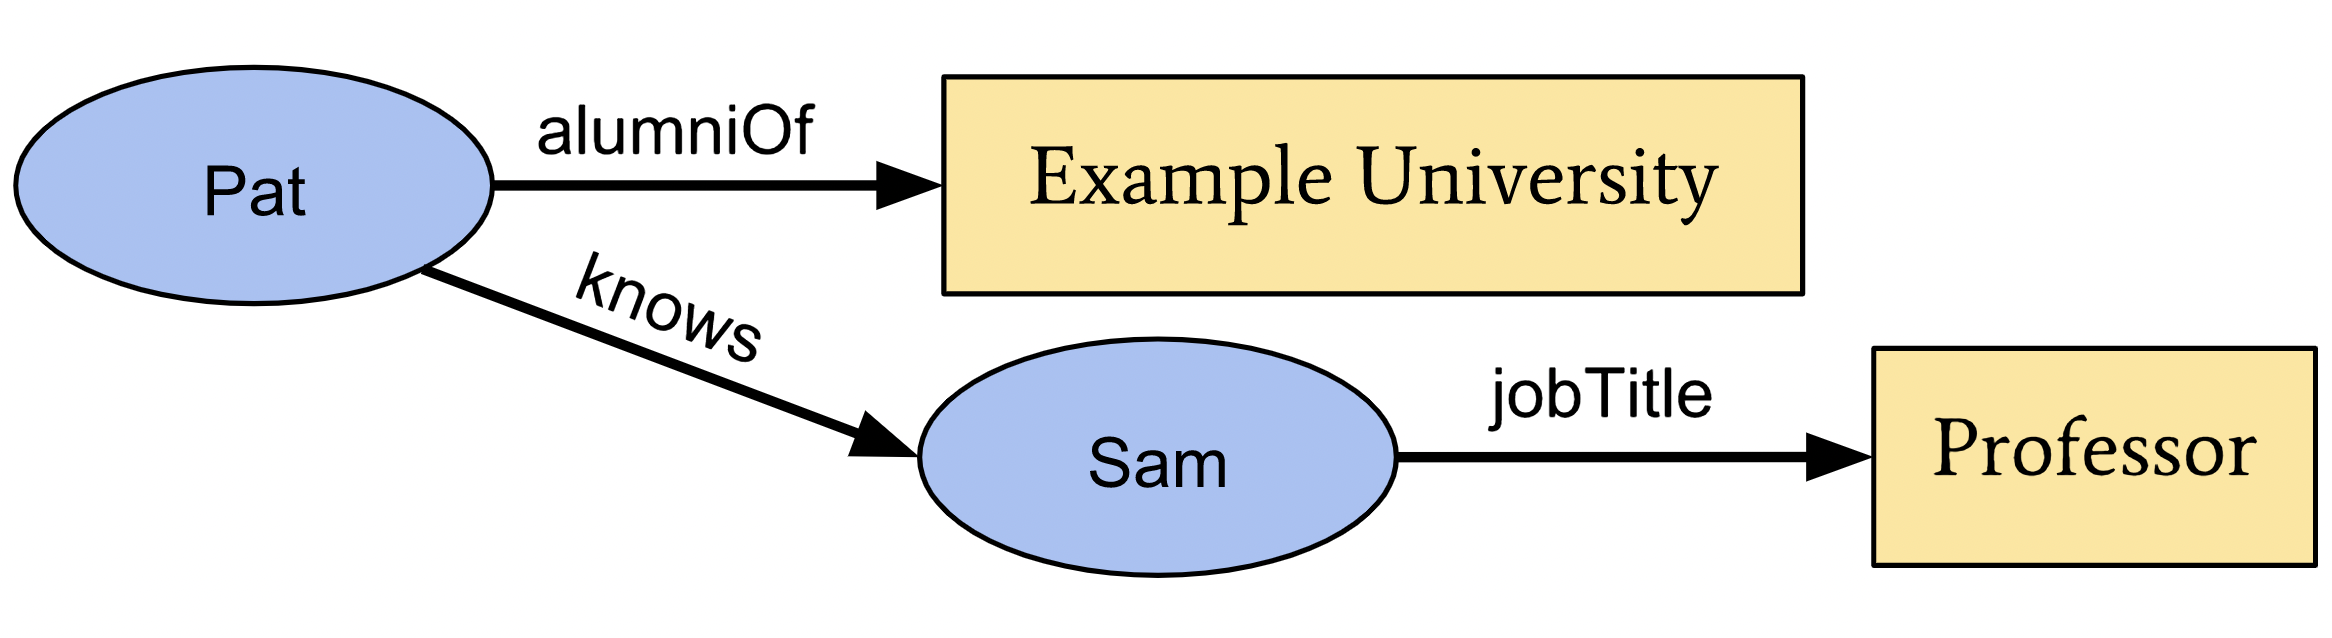
\includegraphics[width=1\textwidth]{figures/claims-example.png}
  \caption{\textit{https://www.w3.org/TR/vc-data-model/#claims}}
\end{figure}








\newpage

\section{Agents and Wallets}

An application which implements \acrshort{ssi}-standards is often called an agent or a wallet.

\begin{figure}[htbp]
  \centering
  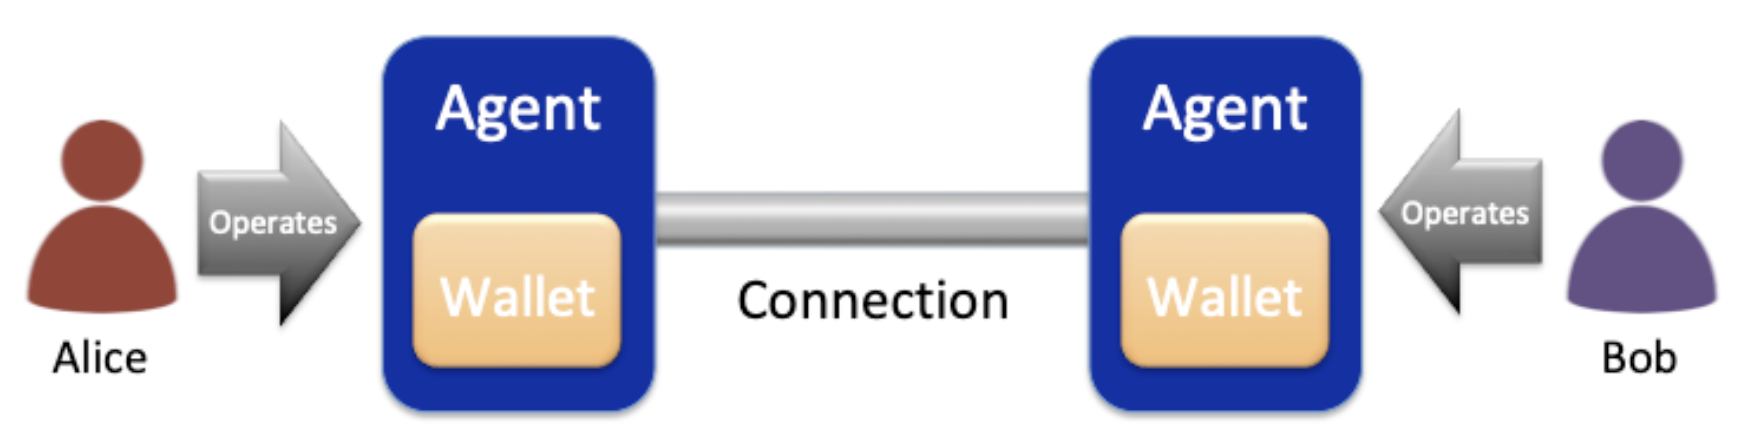
\includegraphics[width=1\textwidth]{figures/agents-and-wallets.png}
  \caption{\textit{https://livebook.manning.com/book/self-sovereign-identity/chapter-2/v-5/}}
\end{figure}


\subsection{Agents}

\begin{itemize}
    \item An agent is a piece of software that is acting on behalf of a \acrshort{did}.
    \item An agent implements one or more of the \acrshort{didcomm}-protocols.
    \item An agent is active. It wants to do things.
\end{itemize}


\subsection{Wallets}

\begin{itemize}
    \item May store \acrfull{vc}.
    \item May store a \acrshort{did}s cryptographic material.
    \item A wallet is passive. It wants to hold things.
\end{itemize}

\subsection{Agents vs Wallets}

In any \acrshort{ssi} discussion these two terms may be used interchangeably about the same app. This is because many instances of \acrshort{ssi}-apps are both an agent and a wallet at the same time. It just depends on the context of the discussion how you refer to the app. If the discussion is about storing credentials and your DIDs, it is more natural to think about the app as a wallet. If the discussion is about issuing, signing, communicating, transfering, validating the best metaphor is to think about the app as an agent.



\newpage

\section{Project Initiator - Diwala}

Diwala is this projects initiator, represented by Snorre Lothar von Gohren. He is the CTO \& Co-Founder of Diwala, which is a for-profit company set out to "build an ecosystem of digital skill identities with verifiable credentials"\cite{DiwalaAbout}.

Snorre also founded \acrfull{din} - a network of organizations which "works to promote decentralized identity and highlight how individuals and society is affected by it.

\section{Project Description}

"The project ambition is to build a proof with the existing wallet standards, that it is possible to establish an open and interoperable identity wallet. Or even prove that this is not possible at this moment, because of the lack of certain standards. As part of the bachelor project team will develop a set of proof-of-concept reference implementations that can showcase the interoperability within the existing frameworks and tools that are already out there. Set together the needed pieces to prove that interoperability is possible. The reference implementation of the proof-of-concept, will prove that the user will be able to seamlessly respond to different service proof requests and issuance requests, and to be able to migrate credentials and other user-centric data stored in the users control. The work will begin with existing open source frameworks, as well as closed source service providers with good developer portals for easy testing and verification. The project is language and platform agnostic. The biggest benefit in this is to showcase that the proclaimed panacea for digital identity, is actually possible. This work will rapport on hinders, benefits and possibilities with this ecosystem, and the importance of interoperability" \cite{ProjectDescription} - \textit{Diwala}






\section{Goals}

Based on the projects description it is useful to derive a list of goals for the project:

\begin{itemize}
    \item Build a proof-of-concept \acrshort{ssi}-application that solves a real-world problem.
    \item Prove that the application is inter-operable with other existing \acrshort{ssi}-application.
\end{itemize}




\section{Boundaries}



\subsection{Organizational Boundaries}

\begin{itemize}
    \item Source-code should be open-source.
    \item Source-code should be hosted by DIN-Foundation.
\end{itemize}




\subsection{Technical Boundaries}
Some technical boundaries for the proof-of-concept implementation:

\begin{itemize}
    \item Should be implemented in the Rust programming language.
    \item Use existing Rust libraries wherever possible.
    \item The application should have a \acrfull{cli}.
    \item No \acrfull{gui}.
    \item Only support one DIDComm transport: \acrshort{stdin}/\acrshort{stdout}
    \item Only support one DID-method: \gls{did-key}
    \item Only support one cryptographic-method: x25519/ed25519
    \item The source code should be open-source.
    \item The source code should be hosted by \acrshort{din}'s Github.
\end{itemize}



\section{Target audience}

\subsection{Public institutions}

We want to build the trust in SSI-infrastructure that is need for public institutions to adopt the technology.


\newpage

\section{Team Roles}

The team working on this project consists of a 1 student, 1 product owner, 2 tech supervisors and 1 academic supervisor.

\begin{table}
  \centering
  \caption{Team Roles}
  \label{tab:example1}
  \begin{tabular}{cc}
    \hline
    Name  & Role \\
    \hline
    Jonas       & Leader, Developer, Student         \\
    Snorre      & Product Owner, Tech supervisor \\
    Mariusz     & Tech supervisor \\
    Abylay      & Tech supervisor \\
    Deepti      & Academic supervisor \\
    \hline
  \end{tabular}
\end{table}



\newpage

\section{Proof-of-concept - DID CLI}

The project description demands that a proof-of-concept agent should be developed. This proof-of-concept wallet will now be referred to as \acrfull{did-cli}. Chapter 2-7 are dedicated to describe how \acrshort{did-cli} was developed. Chapter 8-9 tries to take a step back again and answers the more general questions and goals set out by the project description.

\section{Chapters Overview}

\begin{description}
    \item[Chapter 2:] Development Process - How development of \acrshort{did-cli} was managed.
    \item[Chapter 3:] Requirements - The functional and non-functional requirements of \acrshort{did-cli}.
    \item[Chapter 4:] Application Architecture - A description of the high-level design of \acrshort{did-cli}.
    \item[Chapter 5:] Command-Line Interface - A description of the user-interface of \acrshort{did-cli}.
    \item[Chapter 6:] Implementation - Details about \acrshort{did-cli} source-code.
    \item[Chapter 7:] Quality Assurance - How we test and make sure \acrshort{did-cli} does what it is supposed to do. 
    \item[Chapter 8:] Discussion - What did we decide, learn, think, feel?
    \item[Chapter 9:] Conclusion - Summary and future work.
\end{description}
